\chapter{Basi di Dati}

Le \textbf{Basi di Dati (Database)} sono collezioni organizzate di dati che permettono un'efficiente memorizzazione, recupero e gestione delle informazioni. Sono fondamentali per la maggior parte delle applicazioni software moderne.

\section{Modello Concettuale Entità-Relazione (ER)}
Il \textbf{Modello Entità-Relazione (ER)} è uno strumento concettuale di alto livello utilizzato nella fase iniziale della progettazione di database. Permette di rappresentare il mondo reale in termini di "entità" (oggetti o concetti di interesse) e "relazioni" (associazioni tra le entità). L'obiettivo è fornire una rappresentazione intuitiva e facilmente comprensibile della struttura dei dati prima di tradurla in un modello logico.

\subsection{Componenti Base e Rappresentazione Grafica}
I principali componenti del Modello ER sono le entità, gli attributi e le relazioni, ognuno con una specifica rappresentazione grafica che ne facilita la visualizzazione.
\begin{itemize}
    \item \textbf{Entità}: Rappresentano "cose" o "oggetti" del mondo reale su cui si vogliono memorizzare informazioni. Possono essere concrete (es. Persona, Prodotto) o astratte (es. Corso, Ordine). Nel diagramma ER, le entità sono generalmente rappresentate con un rettangolo.
    \item \textbf{Attributi}: Sono le proprietà o caratteristiche che descrivono un'entità o una relazione. Ad esempio, un'entità "Studente" può avere attributi come "Nome", "Cognome", "Matricola". Nel diagramma ER, gli attributi sono rappresentati con un ovale.
    \item \textbf{Relazioni}: Rappresentano associazioni logiche tra due o più entità. Ad esempio, un "Docente" "insegna" a un "Corso". Nel diagramma ER, le relazioni sono rappresentate con un rombo.
\end{itemize}

\subsection{Dettagli degli Attributi e Identificatori}
Gli attributi possono presentare diverse caratteristiche e alcuni di essi assumono un ruolo speciale come identificatori.
\begin{itemize}
    \item \textbf{Tipi di Attributi}:
    \begin{itemize}
        \item \textbf{Attributi Semplici}: Non possono essere scomposti (es. "Età").
        \item \textbf{Attributi Composti}: Formati da più attributi (es. "Indirizzo" composto da "Via", "Civico", "Città").
        \item \textbf{Attributi Mono-valore}: Hanno un singolo valore per istanza (es. "DataNascita").
        \item \textbf{Attributi Multi-valore}: Possono avere più valori (es. "NumeriDiTelefono").
        \item \textbf{Attributi Derivati}: Il loro valore può essere calcolato da altri attributi (es. "Età" derivata da "DataNascita").
    \end{itemize}
    \item \textbf{Chiave (Key Attribute)}: Un attributo (o un insieme di attributi) che identifica in modo univoco ogni istanza di un'entità. Viene tipicamente sottolineato nel diagramma ER.
\end{itemize}

\begin{figure}[h!]
    \centering
    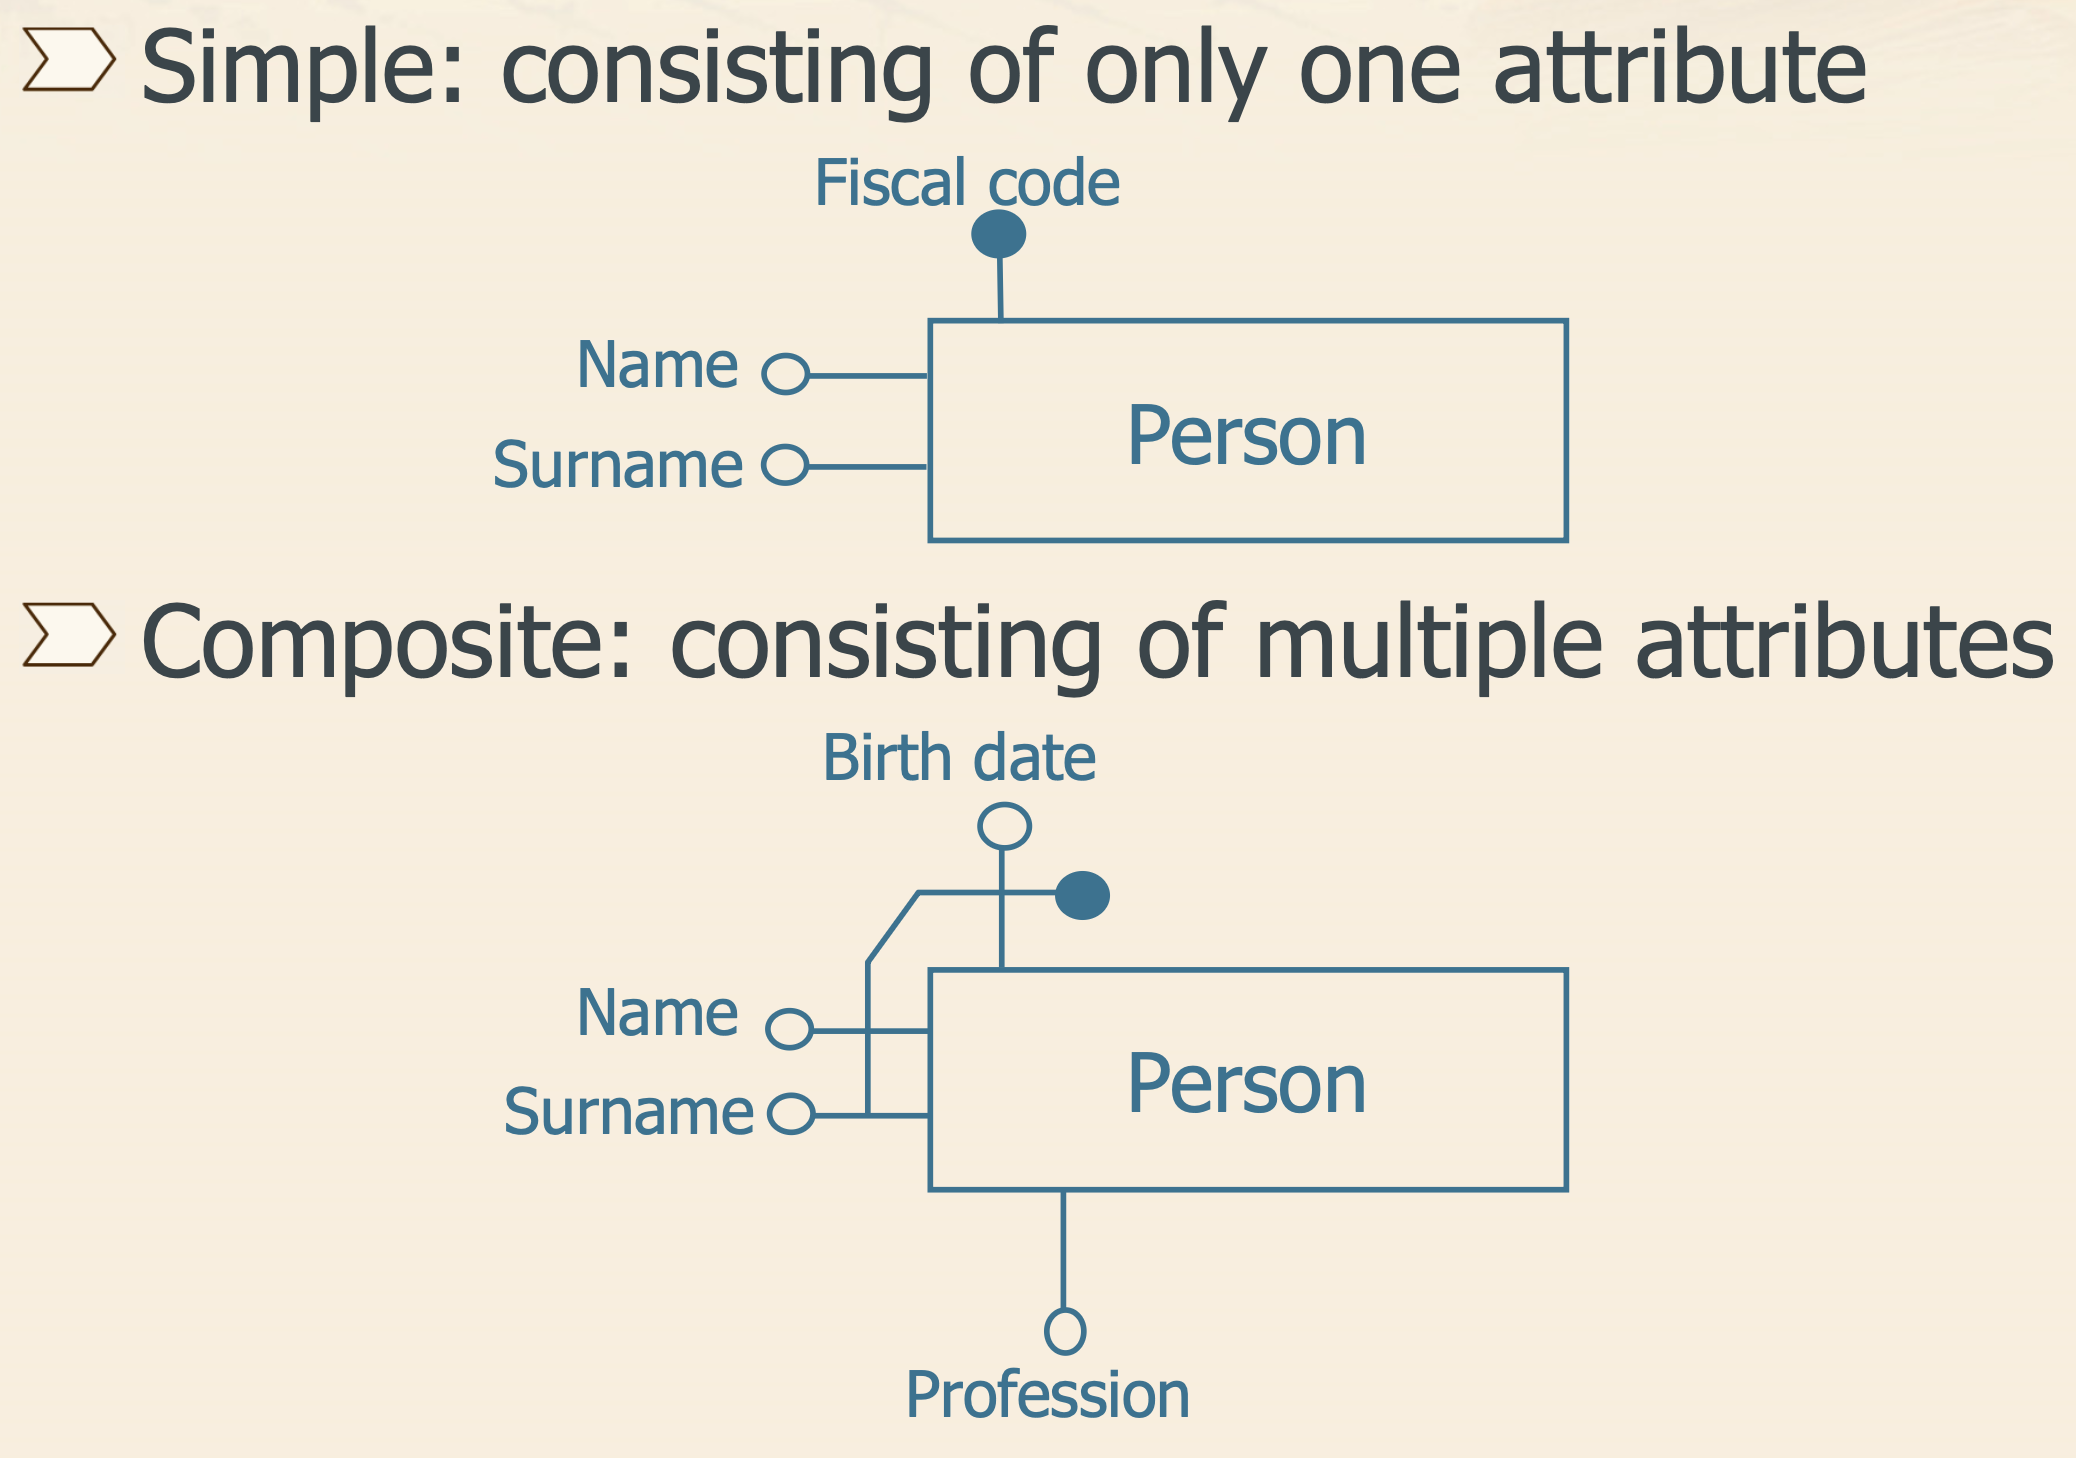
\includegraphics[width=0.7\textwidth]{immagini/er_attributi_semplici_composti.png} 
    \caption{Esempi di rappresentazione di attributi semplici (es. Codice Fiscale) e attributi composti (es. Data di Nascita) in un Diagramma ER.}
    \label{fig:er_attributi_semplici_composti}
\end{figure}

\subsubsection{Identificatori}
Gli identificatori permettono di distinguere univocamente le istanze di un'entità. Possono essere interni o esterni.
\begin{itemize}
    \item \textbf{Identificatore Interno}: Costituito da uno o più attributi dell'entità stessa (es. Codice Fiscale per Persona).
    \item \textbf{Identificatore Esterno}: Coinvolge attributi dell'entità e la partecipazione a relazioni con altre entità, necessarie per la sua identificazione. È tipico delle entità deboli.
\end{itemize}
\begin{figure}[h!]
    \centering
    \subcaptionbox{Identificatore Esterno per Entità Deboli (Studente, Immatricolazione, Università)\label{fig:er_entita_debole_enrollment}}{%
        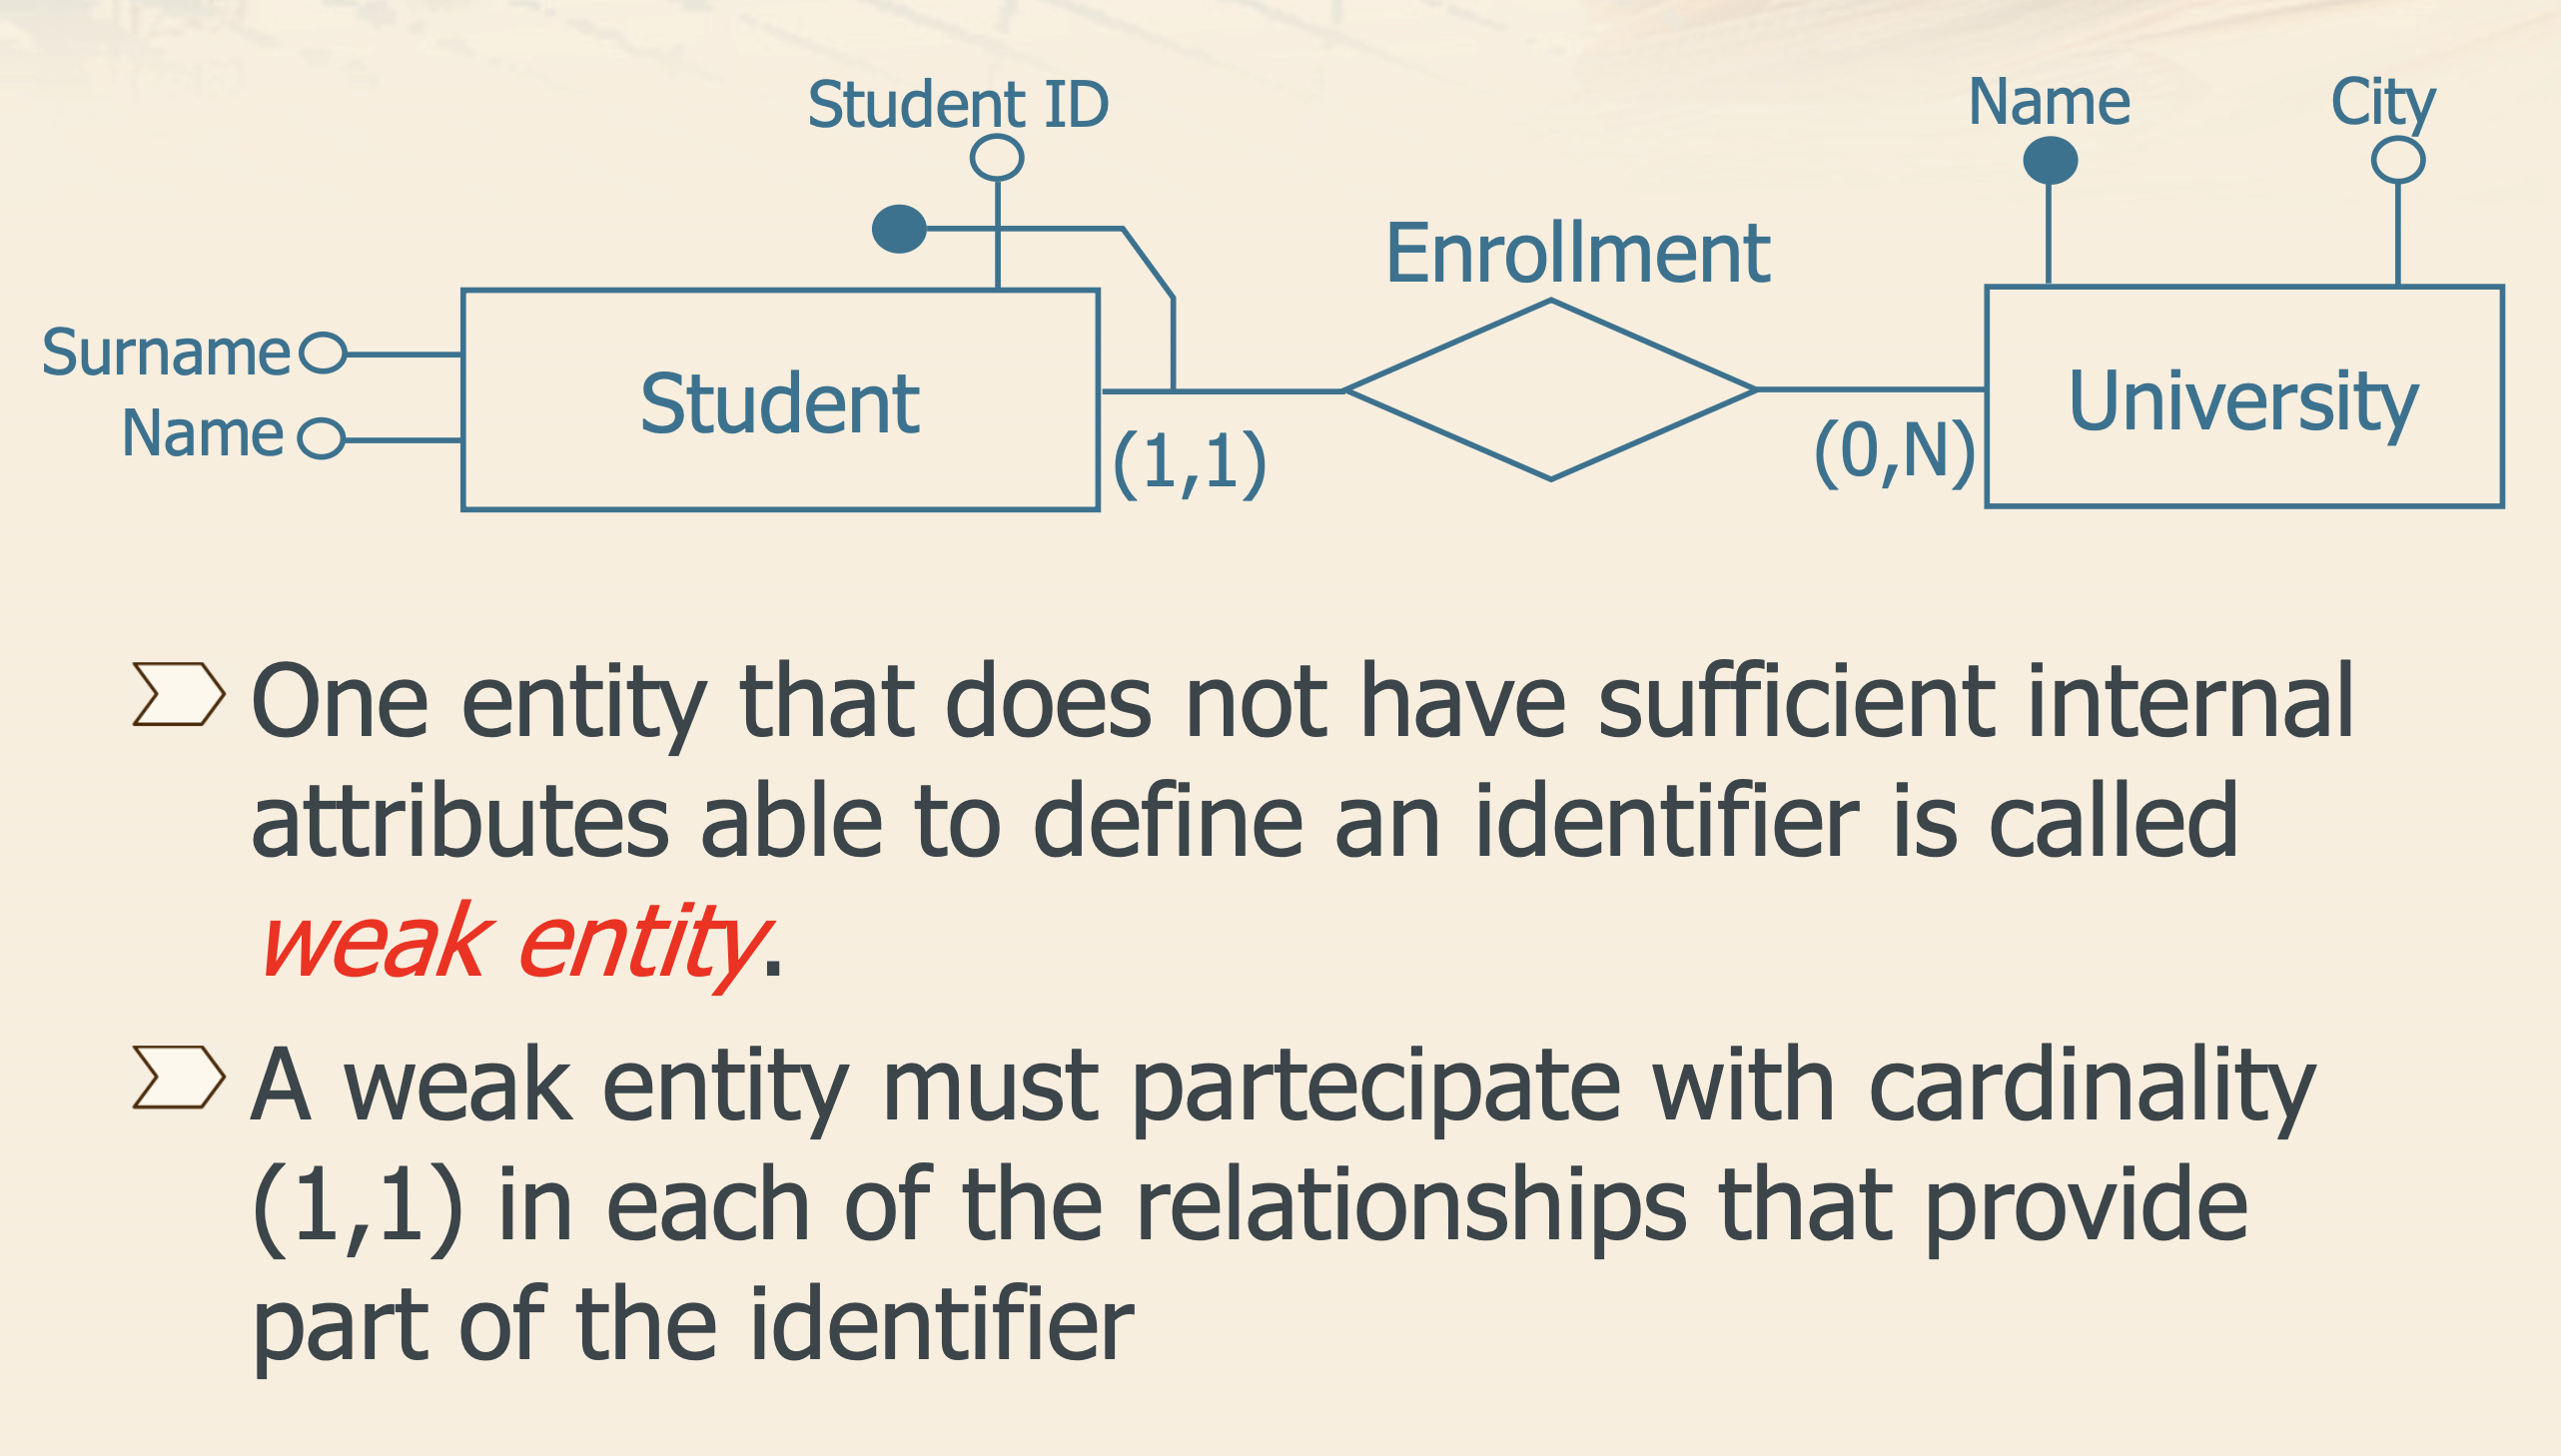
\includegraphics[width=0.48\textwidth]{immagini/er_entita_debole_enrollment.png}%
    }\quad
    \subcaptionbox{Identificatore Esterno Complesso (Stanza, Scaffale, Ripiano)\label{fig:er_identificatore_esterno_libreria}}{%
        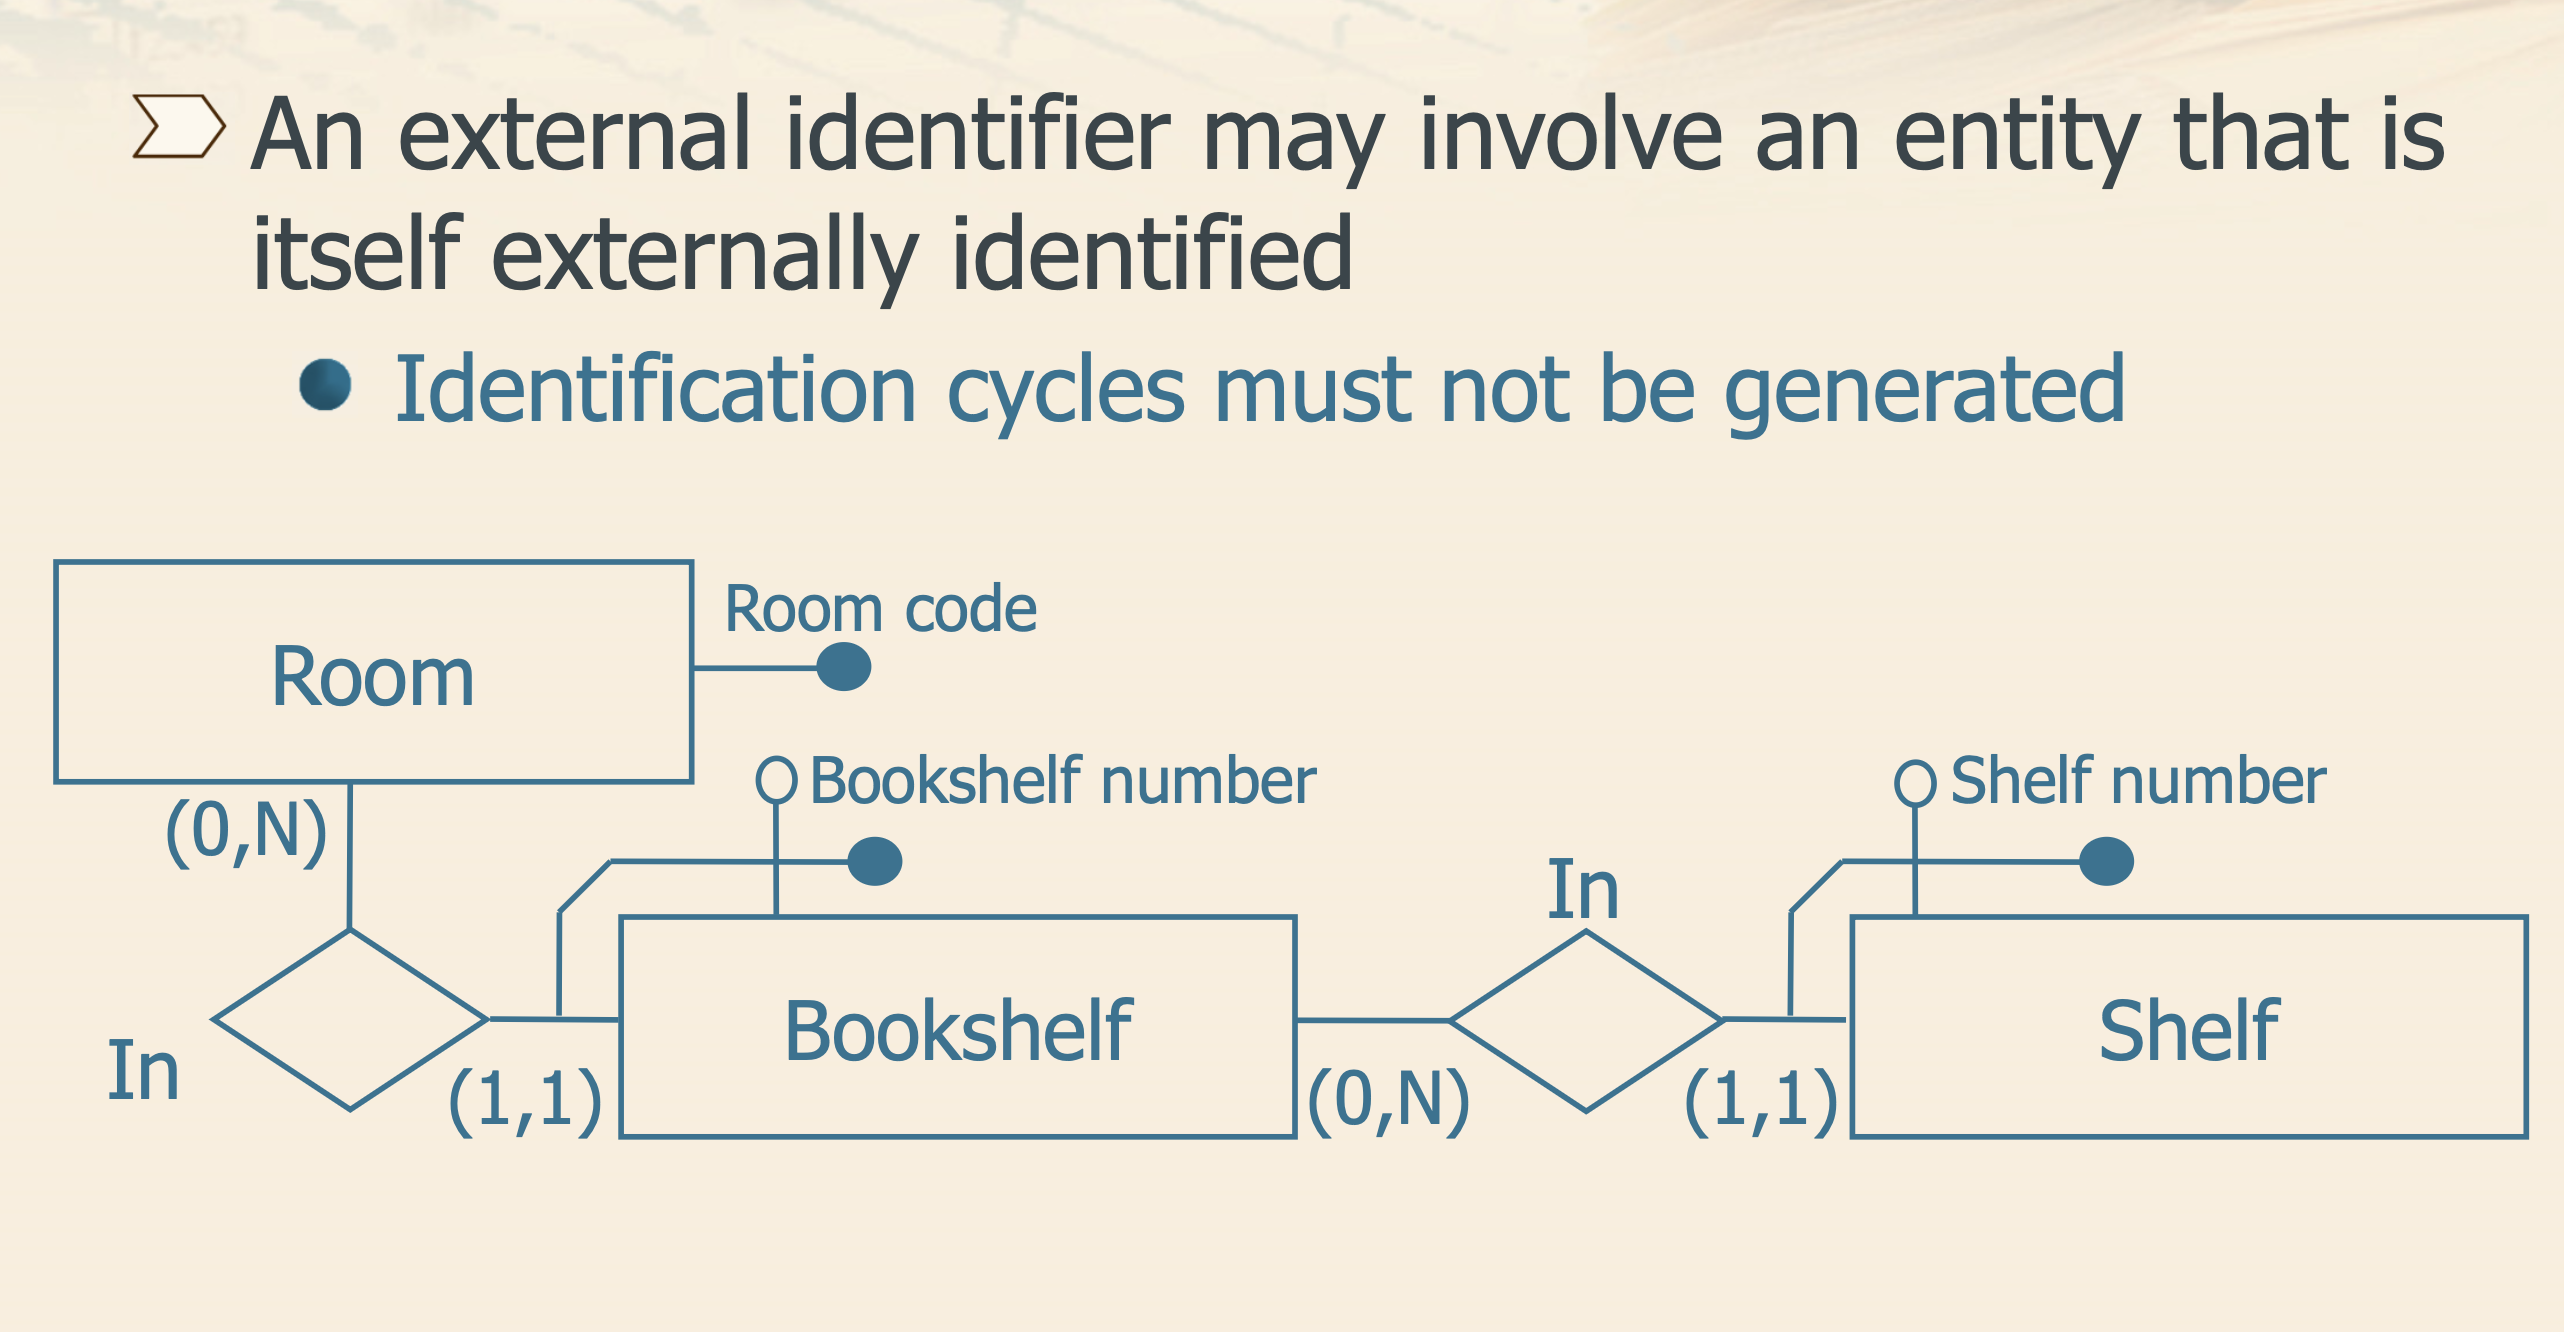
\includegraphics[width=0.48\textwidth]{immagini/er_identificatore_esterno_libreria.png}%
    }
    \caption{Esempi di utilizzo di identificatori esterni, inclusi scenari con entità deboli e concatenazione di identificazione.}
    \label{fig:er_identificatori_esterni}
\end{figure}

\subsection{Dettagli delle Relazioni e Cardinalità}
Le relazioni specificano le associazioni tra le entità, e le cardinalità definiscono il numero di istanze di un'entità che possono partecipare a una relazione.
\begin{itemize}
    \item \textbf{Cardinalità delle Relazioni}: Definisce il numero minimo e massimo di istanze di un'entità che possono essere associate a un'istanza dell'altra entità nella relazione.
    \begin{itemize}
        \item \textbf{Minima}: Indica se la partecipazione è obbligatoria (1) o opzionale (0).
        \item \textbf{Massima}: Indica il numero massimo di partecipazioni (1 o N).
        \item \textbf{Notazione (min, max)}: Es. $(0, N)$ per zero a molti, $(1, N)$ per uno a molti.
    \end{itemize}
    \item \textbf{Partecipazione (o Dipendenza)}:
    \begin{itemize}
        \item \textbf{Totale (o Obbligatoria)}: Ogni istanza dell'entità deve partecipare alla relazione (indicata graficamente da una doppia linea di connessione).
        \item \textbf{Parziale (o Opzionale)}: Un'istanza dell'entità può partecipare o meno alla relazione (indicata graficamente da una singola linea).
    \end{itemize}
\end{itemize}

\subsection{Generalizzazione nel Modello ER}
La \textbf{Generalizzazione} è un costrutto del modello ER che permette di rappresentare una relazione "è un tipo di" (is-a) tra un'entità genitore (generale) e una o più entità figlie (specializzate).
\begin{itemize}
    \item Ogni istanza di un'entità figlia è anche un'istanza dell'entità genitore.
    \item Le proprietà (attributi, identificatori, relazioni) dell'entità genitore sono ereditate da tutte le entità figlie.
\end{itemize}
\begin{figure}[h!]
    \centering
    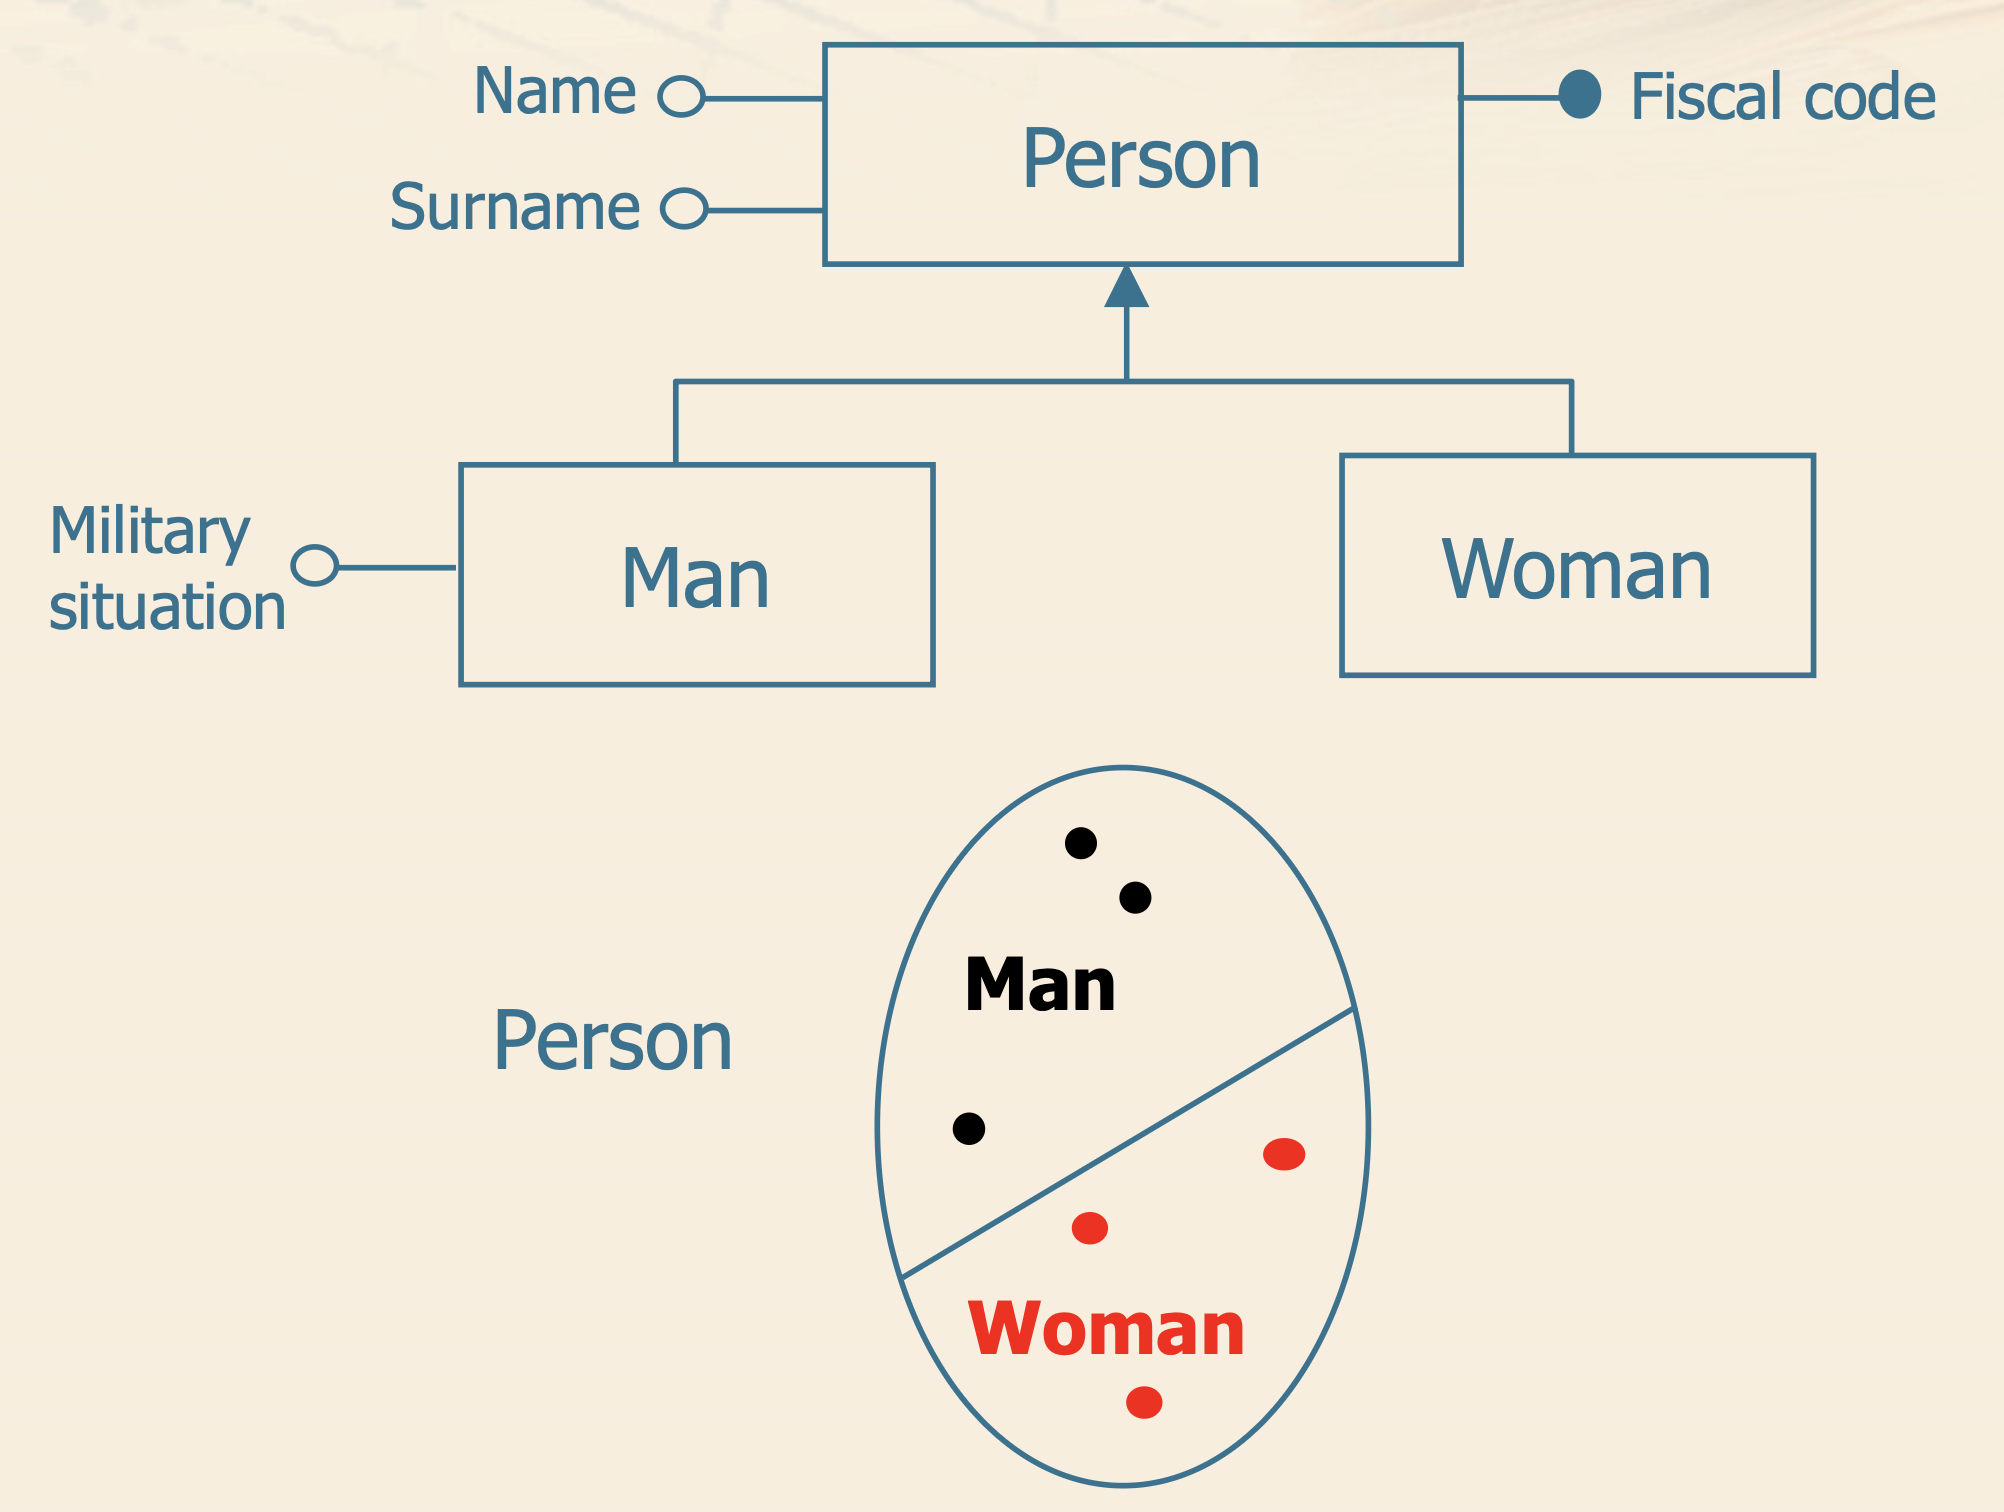
\includegraphics[width=0.7\textwidth]{immagini/er_generalizzazione_person_gender.png} % Immagine dal tuo screenshot 16.08.24.jpg
    \caption{Esempio di Generalizzazione nel Diagramma ER: l'entità Persona si generalizza nelle entità Uomo e Donna, mostrando la distinzione e l'ereditarietà delle proprietà.}
    \label{fig:er_generalizzazione_person_gender}
\end{figure}

\subsection{Esempi Complessi di Schemi ER}
Per consolidare la comprensione del Modello ER, è utile analizzare esempi complessi che integrano vari concetti come entità, attributi, relazioni con cardinalità diverse, identificatori, generalizzazioni e entità deboli. Questi schemi rappresentano contesti reali e mostrano come i costrutti ER vengono applicati per modellare domini complessi.

\begin{figure}[h!]
    \centering
    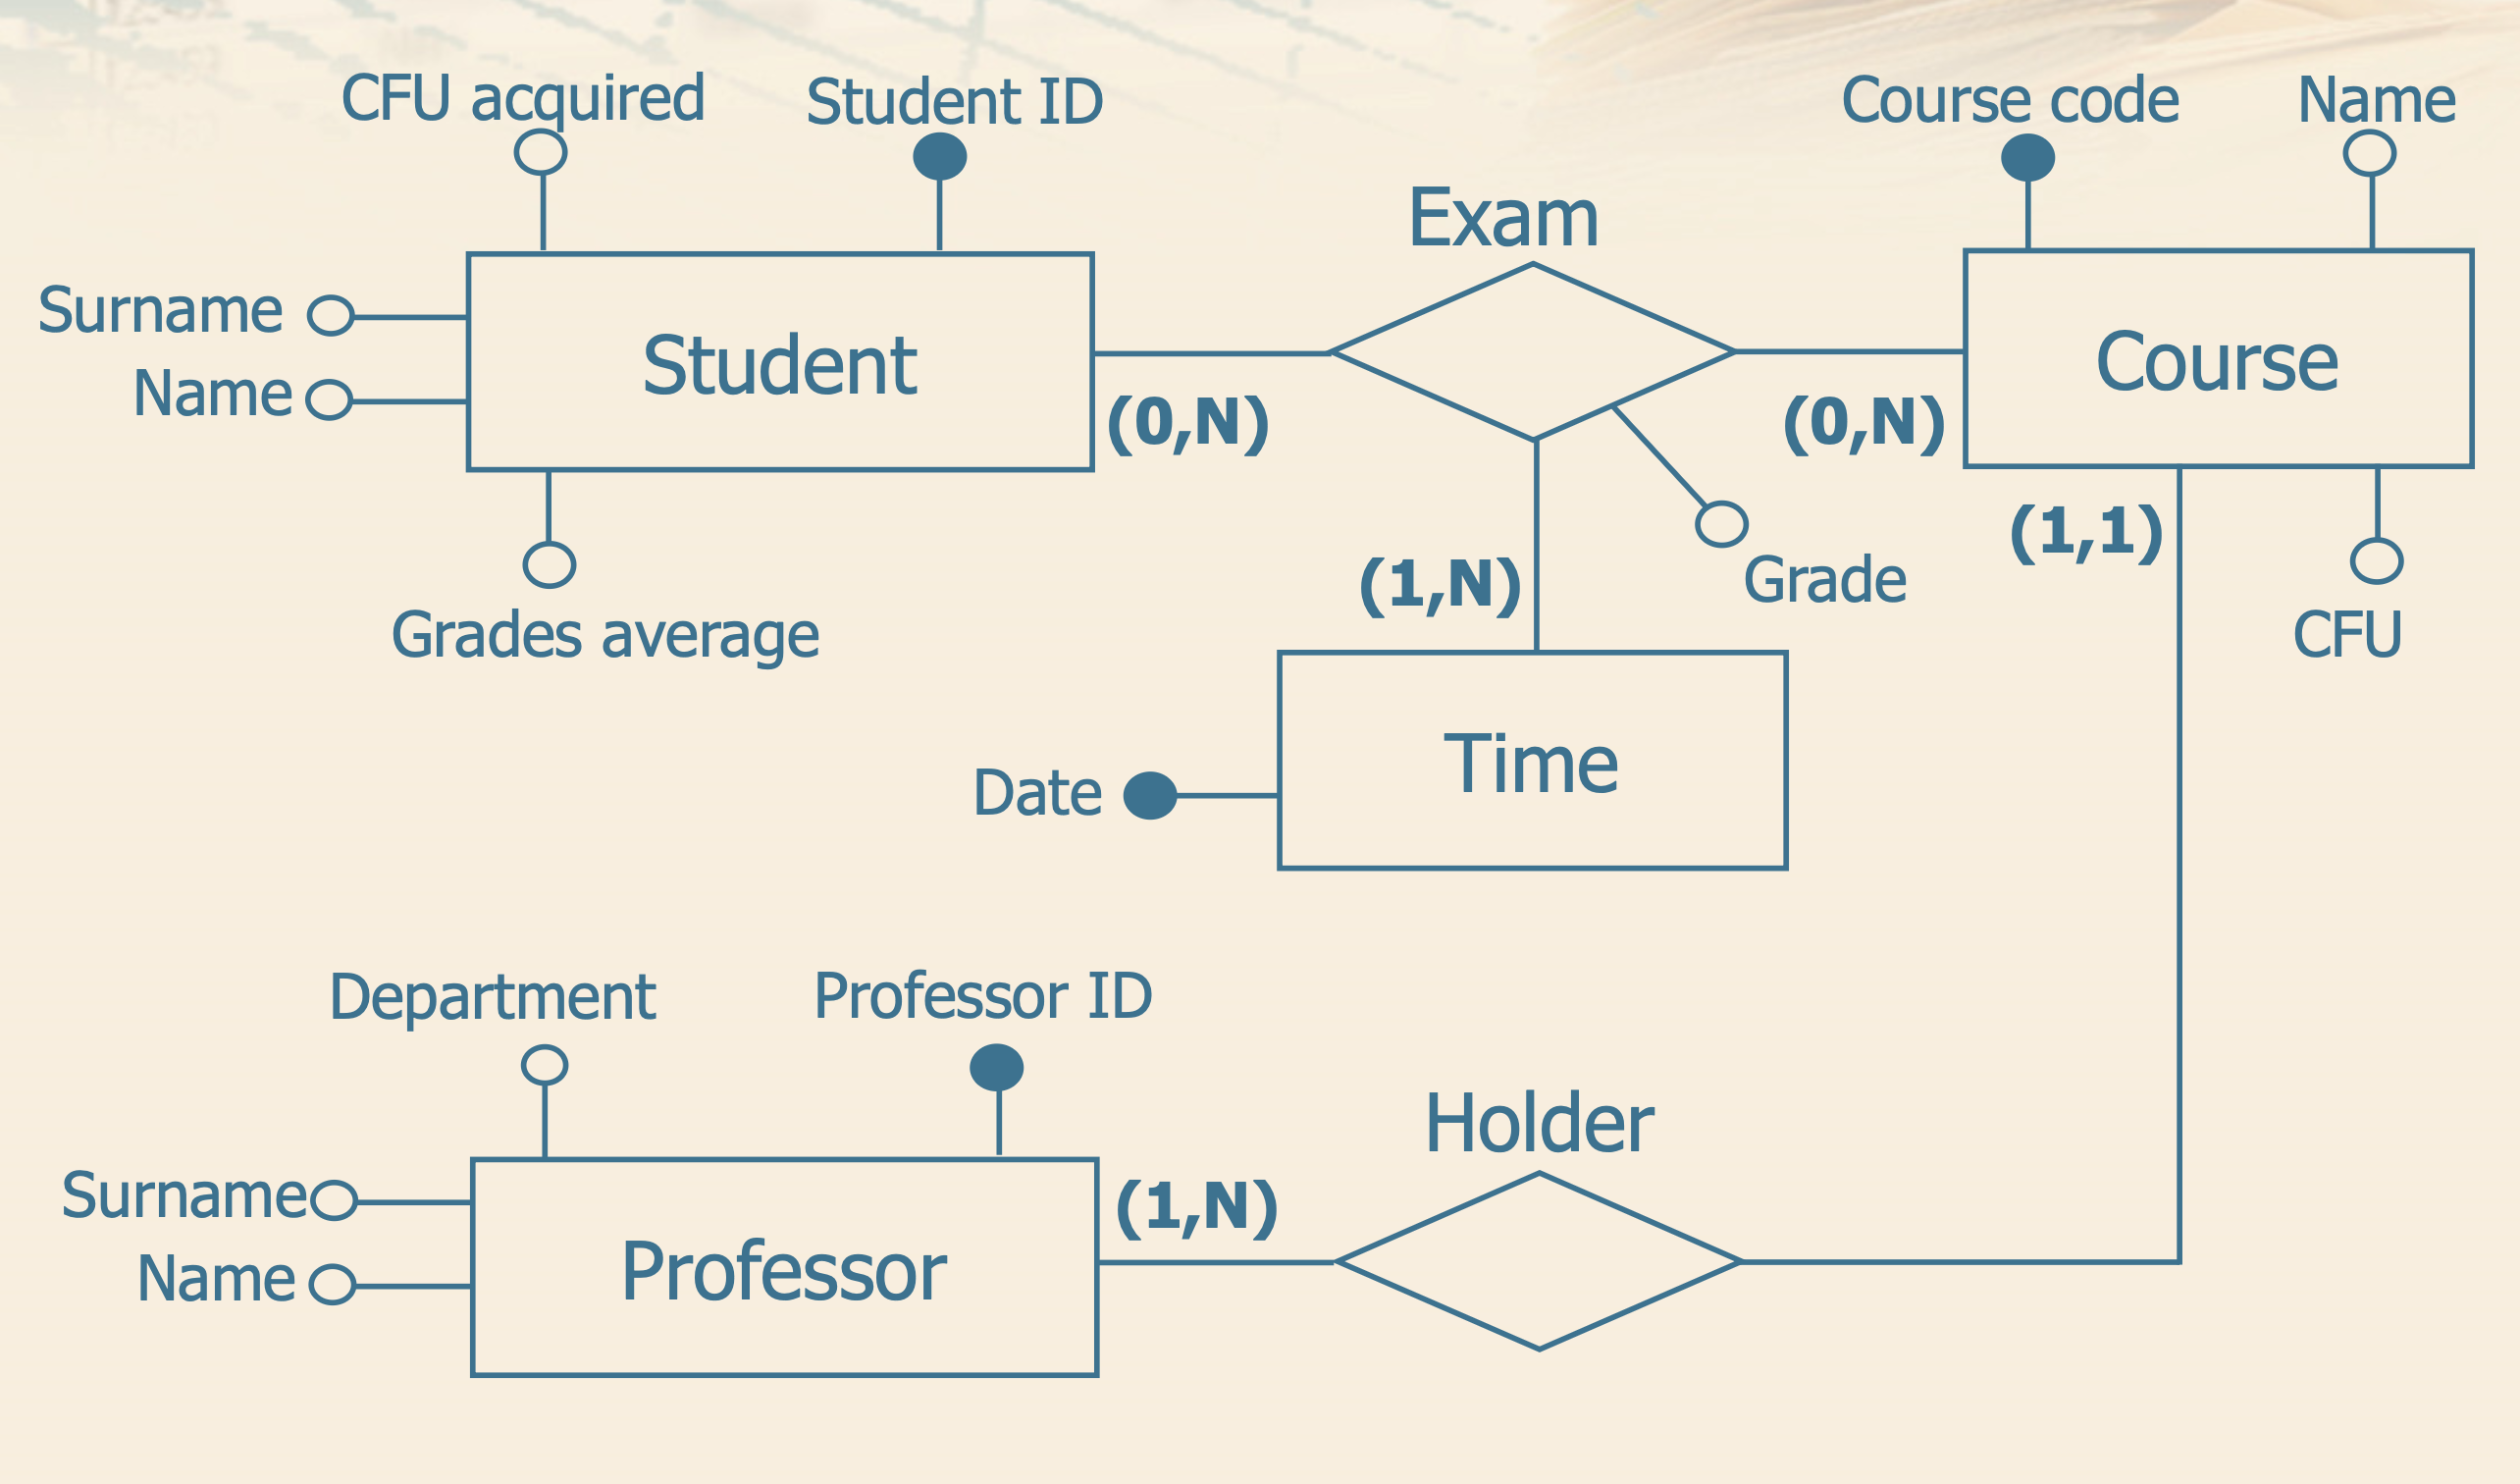
\includegraphics[width=0.9\textwidth]{immagini/er_schema_student_course_exam.png} % Immagine dal tuo screenshot 16.09.49.jpg
    \caption{Diagramma ER che modella le relazioni tra Studenti, Corsi ed Esami, inclusi attributi e cardinalità.}
    \label{fig:er_schema_student_course_exam}
\end{figure}

\subsection{Esempi Complessi di Schemi ER}
Per consolidare la comprensione del Modello ER, è utile analizzare esempi complessi che integrano vari concetti come entità, attributi, relazioni con cardinalità diverse, identificatori, generalizzazioni e entità deboli. Questi schemi rappresentano contesti reali e mostrano come i costrutti ER vengono applicati per modellare domini complessi.

\begin{figure}[h!]
    \centering
    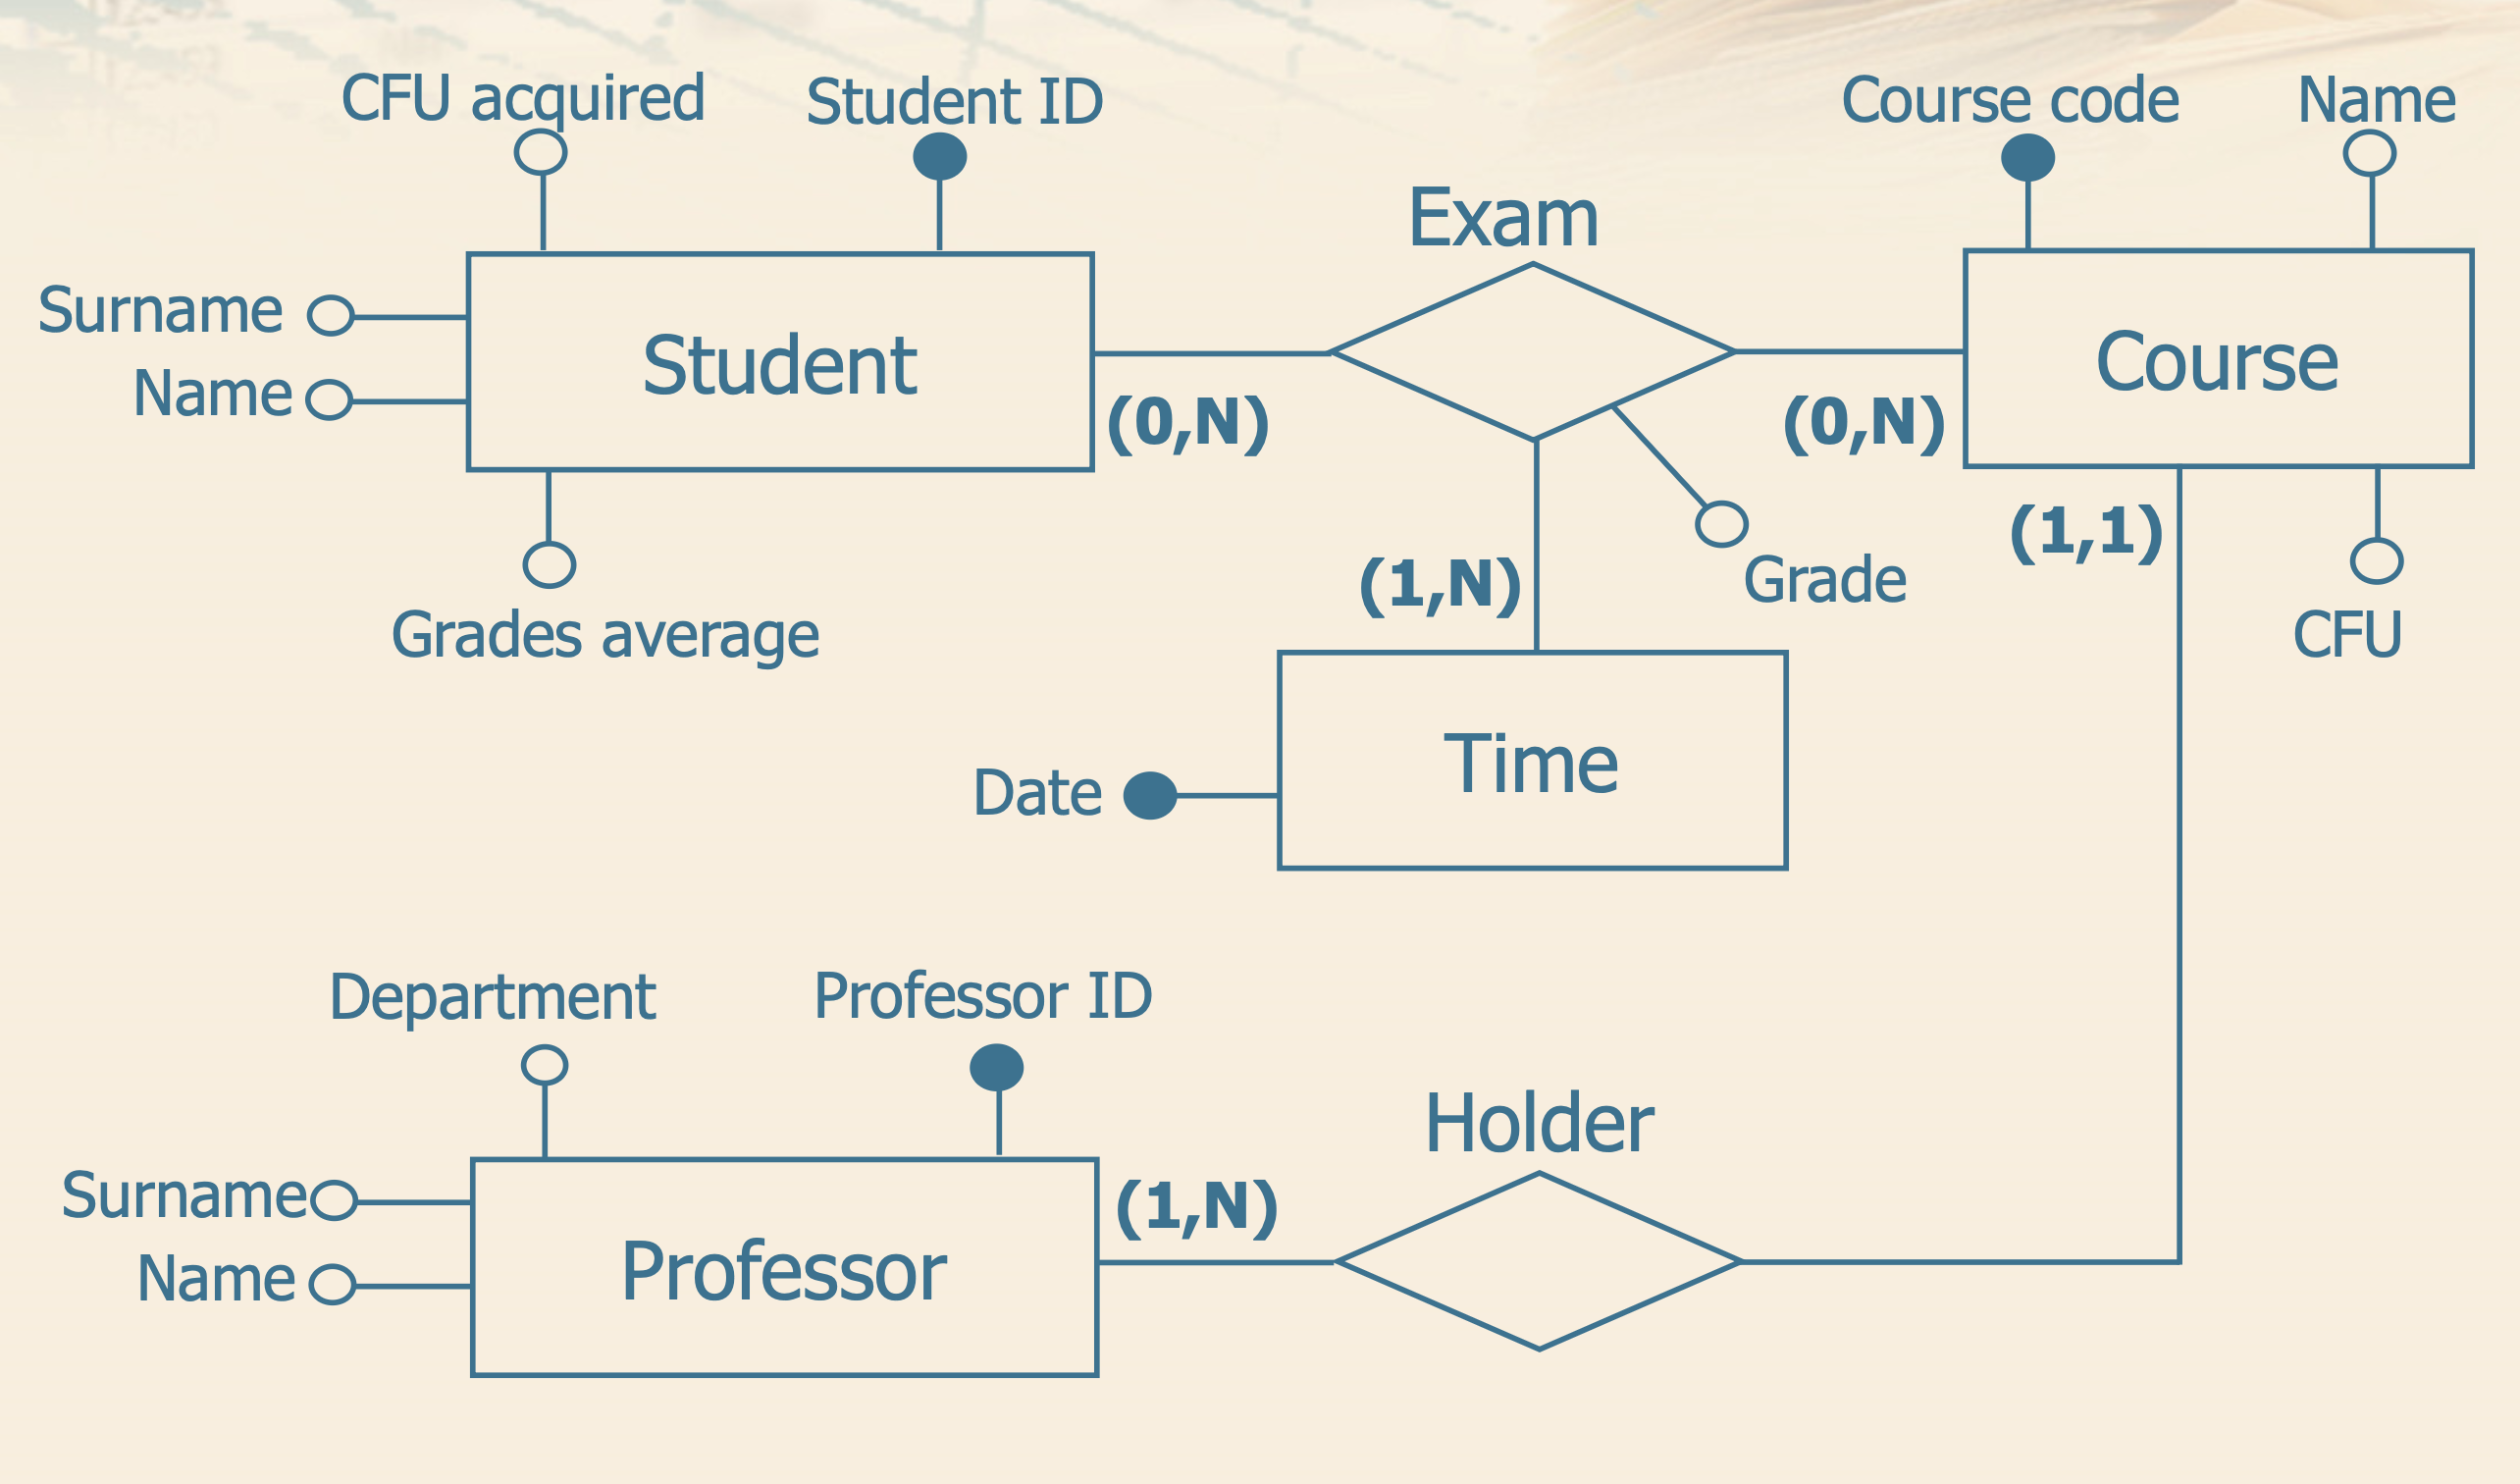
\includegraphics[width=0.9\textwidth]{immagini/er_schema_student_course_exam.png} % Immagine dal tuo screenshot 16.09.49.jpg
    \caption{Diagramma ER che modella le relazioni tra Studenti, Corsi ed Esami, inclusi attributi e cardinalità.}
    \label{fig:er_schema_student_course_exam}
\end{figure}

\subsubsection{Esercizio 2: Sistema Cinema/Film}
\textbf{Descrizione}: Si consideri uno schema Entità-Relazione che rappresenta un sistema per la gestione di film, artisti, cinema e città. Il diagramma include entità come Film, Artista, Cinema e Città, con relazioni che specificano la regia, l'interpretazione e la proiezione dei film nei cinema locali.
\begin{figure}[h!]
    \centering
    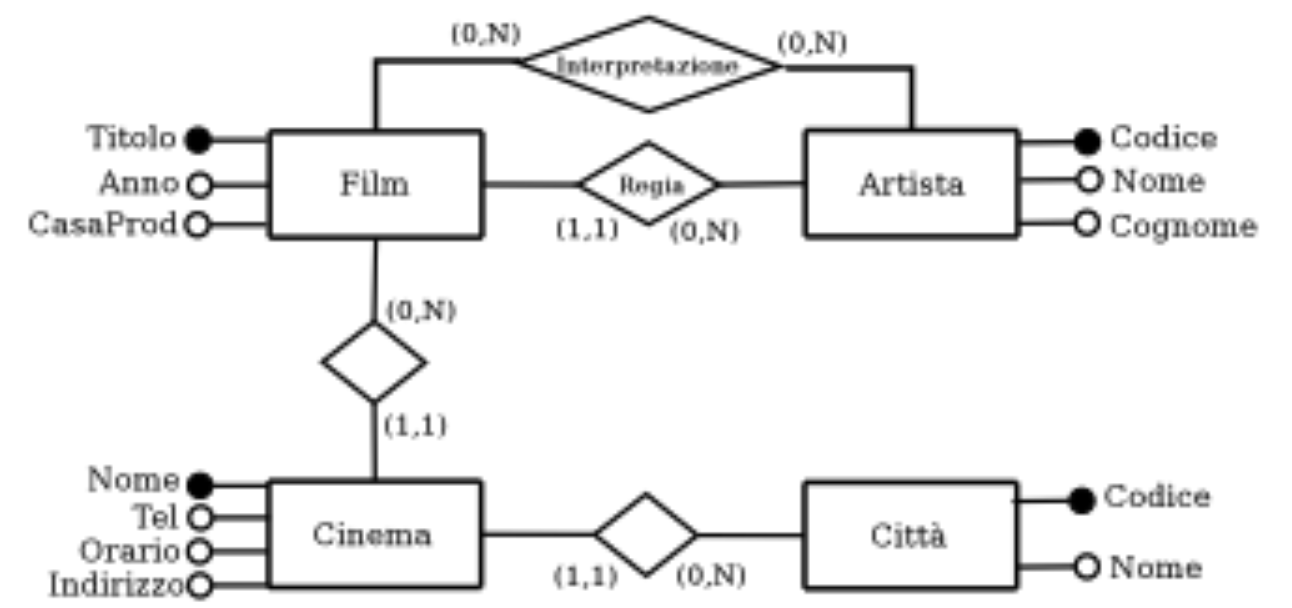
\includegraphics[width=0.9\textwidth]{immagini/er_esercizio_2_cinema_film.png} % Immagine da eserciziER.pdf, Pagina 1, Figura 1
    \caption{Schema ER per l'esercizio 2: Sistema Cinema/Film.}
    \label{fig:er_esercizio_2_cinema_film}
\end{figure}

\textbf{Schema Relazionale corrispondente}:
\begin{lstlisting}[language=SQL]
ARTISTI (Codice, Nome, Cognome)
FILM (Titolo, Anno, CasaProduttrice, RegistaArtista) -- RegistaArtista FK a ARTISTI
INTERPRETAZIONI (FilmTitolo, FilmAnno, ArtistaCodice) -- FK a FILM, FK a ARTISTI
CITTA (Codice, Nome)
CINEMA (Nome, Tel, Orario, Indirizzo, CittaCodice) -- CittaCodice FK a CITTA
PROIEZIONI (FilmTitolo, FilmAnno, CinemaNome, OrarioCinema) -- FK a FILM, FK a CINEMA
\end{lstlisting}

\subsubsection{Esercizio 7: Sistema Campionato di Calcio}
\textbf{Descrizione}: Modellare un sistema per la gestione di un campionato di calcio. Il sistema deve rappresentare squadre, giocatori (con i loro ruoli e dati personali), arbitri, giornate e partite, inclusi i risultati e le specificità come partite in campo neutro o rinviate.
\begin{figure}[h!]
    \centering
    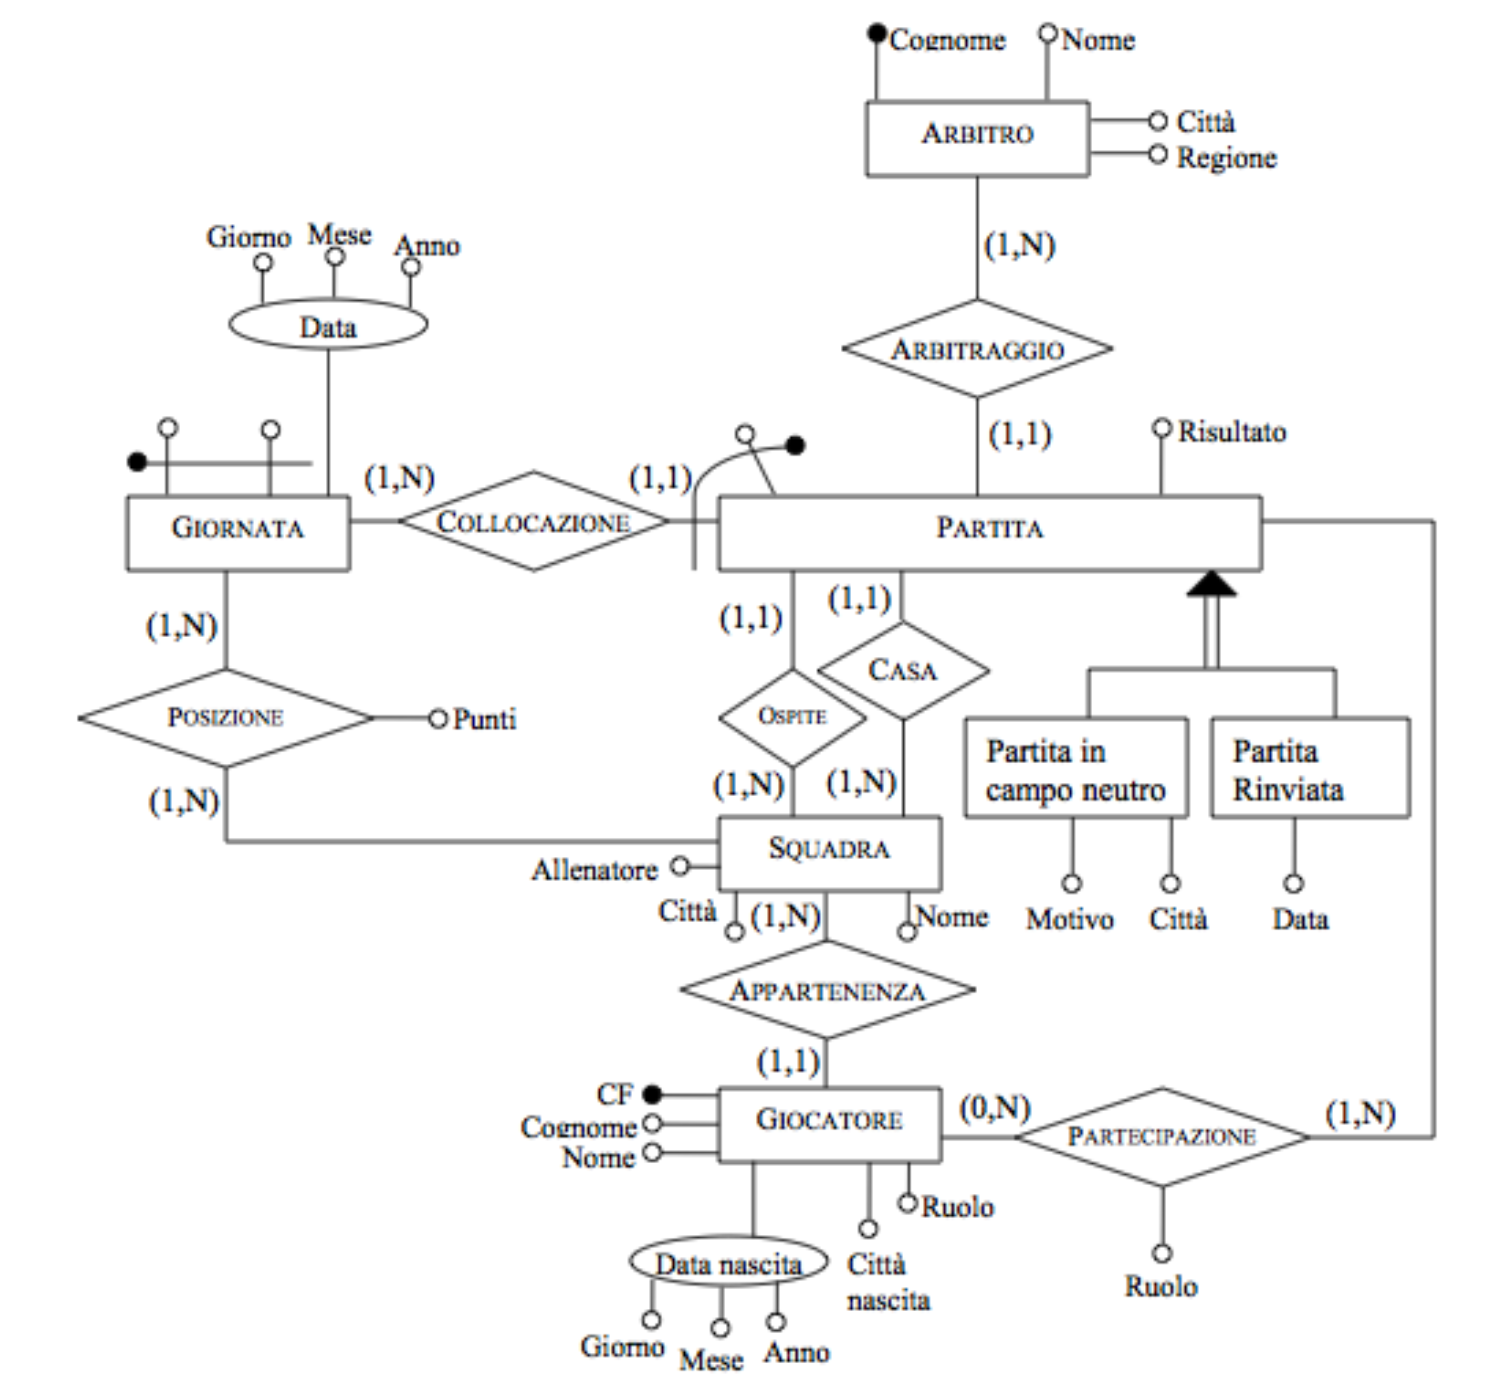
\includegraphics[width=0.9\textwidth]{immagini/er_esercizio_7_campionato_calcio.png} % Immagine da eserciziER.pdf, Pagina 3, Figura 6
    \caption{Schema ER per l'esercizio 7: Sistema Campionato di Calcio.}
    \label{fig:er_esercizio_7_campionato_calcio}
\end{figure}

\textbf{Schema Relazionale corrispondente}:
\begin{lstlisting}[language=SQL]
ARBITRO (Cognome, Nome, Citta, Regione) -- Chiave primaria (Cognome, Nome) o ID_Arbitro generato
GIORNATA (Numero, Serie, Giorno, Mese, Anno) -- Chiave primaria (Numero, Serie)
SQUADRA (Nome, Citta, Allenatore) -- Chiave primaria (Nome)
GIOCATORE (CodiceFiscale, Cognome, Nome, Ruolo, CittaDiNascita) -- Chiave primaria (CodiceFiscale)
PARTITA (NumeroPartita, GiornoGiornata, MeseGiornata, AnnoGiornata, Risultato, ArbitroCognome, ArbitroNome, CasaSquadra, OspiteSquadra) -- Chiave primaria (NumeroPartita), FK a GIORNATA, FK a ARBITRO, FK a SQUADRA (due volte)
PARTITA_IN_CAMPO_NEUTRO (PartitaNumero, PartitaGiorno, PartitaMese, PartitaAnno, Motivo, CittaCampoNeutro) -- FK a PARTITA
PARTITA_RINVIATA (PartitaNumero, PartitaGiorno, PartitaMese, PartitaAnno, DataRinvio) -- FK a PARTITA
POSIZIONE (SquadraNome, GiornoGiornata, MeseGiornata, AnnoGiornata, Punteggio) -- Chiave primaria (SquadraNome, GiornoGiornata, MeseGiornata, AnnoGiornata), FK a SQUADRA, FK a GIORNATA
APPARTENENZA (GiocatoreCodiceFiscale, SquadraNome, DataInizio, RuoloPrincipale, DataFine) -- Chiave primaria (GiocatoreCodiceFiscale, SquadraNome, DataInizio), FK a GIOCATORE, FK a SQUADRA
\end{lstlisting}

\subsubsection{Esercizio 11: Sistema Gare Ciclistiche}
\textbf{Descrizione}: Un sistema per la gestione di gare ciclistiche, includendo informazioni su ciclisti, squadre, località, competizioni, edizioni e tappe, con dettagli sulle classifiche e gli orari.
\begin{figure}[h!]
    \centering
    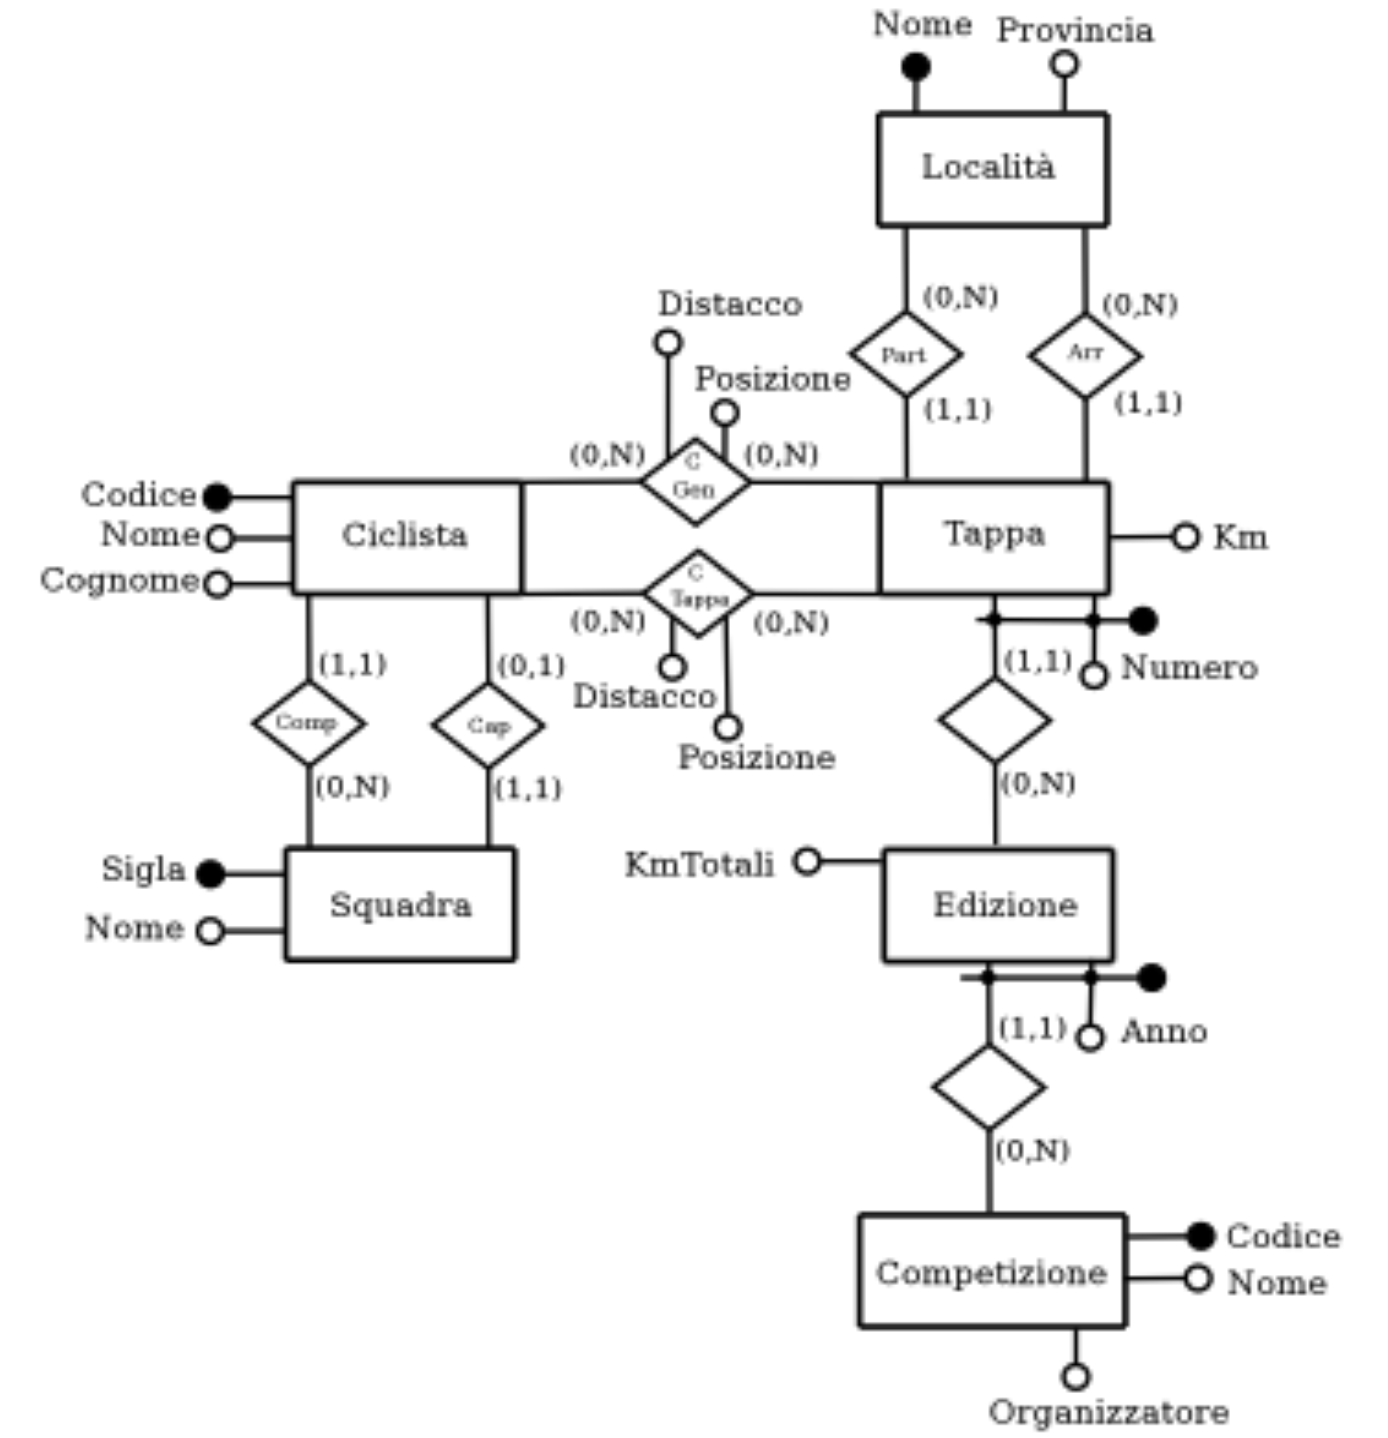
\includegraphics[width=0.9\textwidth]{immagini/er_esercizio_11_ciclisti_tappa.png} % Immagine da eserciziER.pdf, Pagina 5, Figura 10
    \caption{Schema ER per l'esercizio 11: Sistema Gare Ciclistiche.}
    \label{fig:er_esercizio_11_ciclisti_tappa}
\end{figure}

\textbf{Schema Relazionale corrispondente}:
\begin{lstlisting}[language=SQL]
SQUADRE (Sigla, Nome, CapitanoCodice) -- CapitanoCodice FK a CICLISTI
CICLISTI (Codice, Cognome, Nome, SquadraSigla) -- SquadraSigla FK a SQUADRE
LOCALITA (Nome, Provincia) -- Chiave primaria (Nome, Provincia)
COMPETIZIONI (Codice, Nome, Organizzatore) -- Chiave primaria (Codice)
EDIZIONI (AnnoEdizione, CompetizioneCodice, KmTotali) -- Chiave primaria (AnnoEdizione, CompetizioneCodice), FK a COMPETIZIONI
TAPPE (NumeroTappa, AnnoEdizione, CompetizioneCodice, LocPartenzaNome, LocPartenzaProvincia, LocArrivoNome, LocArrivoProvincia) -- Chiave primaria (NumeroTappa, AnnoEdizione, CompetizioneCodice), FK a EDIZIONI, FK a LOCALITA (due volte)
CLASSIFICATAPPA (NumeroTappa, AnnoEdizione, CompetizioneCodice, CiclistaCodice, Posizione, Distacco) -- FK a TAPPE, FK a CICLISTI
CLASSIFICAGENERALE (NumeroTappa, AnnoEdizione, CompetizioneCodice, CiclistaCodice, Posizione, Distacco) -- FK a TAPPE, FK a CICLISTI
\end{lstlisting}

\section{Progettazione Logica: Normalizzazione e Forme Normali}
La \textbf{normalizzazione} è un processo sistematico di organizzazione dei dati in un database relazionale. Il suo scopo è ridurre la ridondanza dei dati, eliminare le anomalie di aggiornamento (inserimento, cancellazione, modifica) e migliorare l'integrità e la coerenza dei dati. La normalizzazione si basa su una serie di regole chiamate "forme normali".

\subsection{Obiettivi della Normalizzazione}
\begin{itemize}
    \item \textbf{Riduzione della Ridondanza}: Evitare la duplicazione inutile dei dati, che spreca spazio e può portare a incongruenze.
    \item \textbf{Miglioramento dell'Integrità dei Dati}: Assicurare che i dati siano accurati e consistenti.
    \item \textbf{Prevenzione delle Anomalie}:
    \begin{itemize}
        \item \textbf{Anomalia di Inserimento}: Impossibilità di inserire un'informazione a meno che non si inseriscano anche altre informazioni non correlate.
        \item \textbf{Anomalia di Cancellazione}: La cancellazione di un dato comporta la perdita accidentale di altre informazioni non desiderate.
        \item \textbf{Anomalia di Aggiornamento}: La modifica di un dato ripetuto richiede l'aggiornamento di più occorrenze, con rischio di inconsistenza se non tutte vengono aggiornate.
    \end{itemize}
    \item \textbf{Flessibilità e Manutenibilità}: Rendere il database più facile da modificare ed estendere.
\end{itemize}

\subsection{Principali Forme Normali}
Le forme normali sono una serie di regole progressive; per essere in una forma normale N, una relazione deve soddisfare i requisiti della forma normale N-1. Le più comuni e rilevanti per la maggior parte delle applicazioni sono la Prima, Seconda e Terza Forma Normale.

\subsubsection{Prima Forma Normale (1NF)}
Una relazione è in 1NF se e solo se:
\begin{itemize}
    \item Tutti gli attributi sono \textbf{atomici} (indivisibili). Non ci sono attributi con valori multipli o attributi composti che non sono stati scomposti.
    \item Ogni record (riga) nella relazione è \textbf{unico}. Questo implica che deve esistere una chiave primaria.
\end{itemize}
\textbf{Esempio di Violazione}: Una colonna "NumeriDiTelefono" che contiene più numeri per un'unica riga.

\subsubsection{Seconda Forma Normale (2NF)}
Una relazione è in 2NF se e solo se:
\begin{itemize}
    \item È in \textbf{1NF}.
    \item Tutti gli attributi non-chiave dipendono \textbf{completamente} dalla chiave primaria. Non ci sono dipendenze parziali, il che significa che nessun attributo non-chiave dipende solo da una parte di una chiave primaria composta.
\end{itemize}
\textbf{Esempio di Violazione}: In una tabella `(IDCorso, IDStudente, NomeCorso, Voto)`, se `(IDCorso, IDStudente)` è la chiave primaria, e `NomeCorso` dipende solo da `IDCorso` (e non da `IDStudente`), allora `NomeCorso` è parzialmente dipendente e viola la 2NF.

\subsubsection{Terza Forma Normale (3NF)}
Una relazione è in 3NF se e solo se:
\begin{itemize}
    \item È in \textbf{2NF}.
    \item Non contiene \textbf{dipendenze transitive}. Ovvero, nessun attributo non-chiave dipende da un altro attributo non-chiave (anziché dipendere direttamente dalla chiave primaria).
\end{itemize}
\textbf{Esempio di Violazione}: In una tabella `(IDImpiegato, NomeImpiegato, Dipartimento, CapoDipartimento)`, se `IDImpiegato` è la chiave primaria e `CapoDipartimento` dipende da `Dipartimento` (che a sua volta dipende da `IDImpiegato`), si ha una dipendenza transitiva.

\subsection{Linguaggio SQL}
Il \textbf{Structured Query Language (SQL)} è il linguaggio standard per la gestione dei sistemi di gestione di database relazionali (RDBMS). Permette di definire, manipolare e controllare i dati.

\subsubsection{Categorie di Comandi SQL}
\begin{itemize}
    \item \textbf{Data Definition Language (DDL)}: Utilizzato per definire e modificare la struttura del database.
    \begin{itemize}
        \item \textbf{CREATE}: Crea database, tabelle, viste, indici, ecc. (es. `CREATE TABLE Studenti (...)`).
        \item \textbf{ALTER}: Modifica la struttura di oggetti esistenti (es. `ALTER TABLE Studenti ADD COLUMN Età INT`).
        \item \textbf{DROP}: Cancella oggetti dal database (es. `DROP TABLE Studenti`).
    \end{itemize}
    \item \textbf{Data Manipulation Language (DML)}: Utilizzato per manipolare i dati all'interno delle tabelle.
    \begin{itemize}
        \item \textbf{SELECT}: Recupera dati da una o più tabelle. È la query più usata.
        \item \textbf{INSERT}: Aggiunge nuove righe a una tabella.
        \item \textbf{UPDATE}: Modifica righe esistenti in una tabella.
        \item \textbf{DELETE}: Rimuove righe da una tabella.
    \end{itemize}
    \item \textbf{Data Control Language (DCL)}: Utilizzato per gestire i permessi di accesso ai dati.
    \begin{itemize}
        \item \textbf{GRANT}: Concede privilegi agli utenti.
        \item \textbf{REVOKE}: Rimuove privilegi dagli utenti.
    \end{itemize}
    \item \textbf{Transaction Control Language (TCL)}: Utilizzato per gestire le transazioni (gruppi di operazioni che devono essere eseguite atomicamente).
    \begin{itemize}
        \item \textbf{COMMIT}: Salva le modifiche di una transazione.
        \item \textbf{ROLLBACK}: Annulla le modifiche di una transazione.
    \end{itemize}
\end{itemize}

\subsubsection{Elementi Comuni delle Query SQL (SELECT)}
La query \texttt{SELECT} è la più potente e versatile, permettendo di interrogare il database.
\begin{itemize}
    \item \textbf{SELECT}: Specifica le colonne da recuperare.
    \begin{itemize}
        \item \texttt{SELECT colonna1, colonna2}
        \item \texttt{SELECT *} (tutte le colonne)
        \item \texttt{SELECT DISTINCT colonna} (solo valori unici)
    \end{itemize}
    \item \textbf{FROM}: Specifica la tabella (o le tabelle) da cui recuperare i dati.
    \item \textbf{WHERE}: Filtra le righe in base a una condizione specificata.
    \begin{itemize}
        \item \texttt{WHERE condizione} (es. `WHERE Età > 18`)
        \item Operatori: `=`, `>`, `<`, `>=`, `<=`, `<>`, `LIKE` (per pattern matching), `IN`, `BETWEEN`, `IS NULL`.
    \end{itemize}
    \item \textbf{JOIN}: Combina righe da due o più tabelle basandosi su una colonna correlata.
    \begin{itemize}
        \item \textbf{INNER JOIN}: Restituisce solo le righe che hanno corrispondenze in entrambe le tabelle.
        \item \textbf{LEFT (OUTER) JOIN}: Restituisce tutte le righe dalla tabella sinistra e le righe corrispondenti dalla tabella destra (con NULL se non ci sono corrispondenze).
        \item \textbf{RIGHT (OUTER) JOIN}: Simile al LEFT JOIN, ma per la tabella destra.
        \item \textbf{FULL (OUTER) JOIN}: Restituisce tutte le righe quando c'è una corrispondenza in una delle due tabelle.
    \end{itemize}
    \item \textbf{GROUP BY}: Raggruppa le righe che hanno gli stessi valori in una o più colonne, spesso usato con funzioni di aggregazione.
    \item \textbf{HAVING}: Filtra i gruppi creati da `GROUP BY` in base a una condizione. Si usa con le funzioni di aggregazione.
    \item \textbf{ORDER BY}: Ordina il set di risultati in base a una o più colonne (ASC per ascendente, DESC per discendente).
    \item \textbf{Funzioni di Aggregazione}: Calcolano un singolo valore da un insieme di valori (es. `COUNT()`, `SUM()`, `AVG()`, `MAX()`, `MIN()`).
\end{itemize}

\subsubsection{Esempi di Operatori e Funzioni SQL Comuni}
Oltre agli elementi base delle query \lstinline{SELECT}, SQL offre un'ampia gamma di operatori e funzioni per manipolare e filtrare i dati in modo più complesso.
\begin{itemize}
    \item \textbf{Operatori Logici}:
    \begin{itemize}
        \item \lstinline{AND}: Combina due condizioni, entrambe devono essere vere.
        \item \lstinline{OR}: Combina due condizioni, almeno una deve essere vera.
        \item \lstinline{NOT}: Nega una condizione.
    \end{itemize}
    \begin{lstlisting}[language=SQL, caption={Esempio Operatori Logici}]
SELECT FirstName, LastName
FROM Students
WHERE Age > 20 AND City = 'Bologna';
    \end{lstlisting}
    \item \textbf{Operatori di Confronto}:
    \begin{itemize}
        \item \lstinline{=}: Uguale a.
        \item \lstinline{<>} o \lstinline{!=}: Diverso da.
        \item \lstinline{<}, \lstinline{>}, \lstinline{<=}, \lstinline{>=}: Minore, maggiore, minore o uguale, maggiore o uguale.
        \item \lstinline{BETWEEN min AND max}: Valore compreso in un intervallo (inclusi gli estremi).
        \item \lstinline{LIKE pattern}: Ricerca stringhe che corrispondono a un pattern (es. \lstinline{LIKE 'A%'}).
        \item \lstinline{IN (value1, value2, ...)}: Valore presente in una lista di valori.
        \item \lstinline{IS NULL} / \lstinline{IS NOT NULL}: Verifica se un valore è NULL.
    \end{itemize}
    \begin{lstlisting}[language=SQL, caption={Esempio Operatori di Confronto}]
SELECT ProductName, Price
FROM Products
WHERE Price BETWEEN 10.00 AND 50.00
  AND ProductName LIKE 'Book%';

SELECT OrderID
FROM Orders
WHERE DeliveryDate IS NULL;
    \end{lstlisting}
    \item \textbf{Funzioni Stringa}:
    \begin{itemize}
        \item \lstinline{CONCAT(s1, s2, ...)}: Concatena stringhe.
        \item \lstinline{SUBSTRING(string, start, length)}: Estrae una sottostringa.
        \item \lstinline{LENGTH(string)}: Restituisce la lunghezza di una stringa.
        \item \lstinline{UPPER(string)} / \lstinline{LOWER(string)}: Converte in maiuscolo/minuscolo.
    \end{itemize}
    \begin{lstlisting}[language=SQL, caption={Esempio Funzioni Stringa}]
SELECT CONCAT(FirstName, ' ', LastName) AS FullName
FROM Users
WHERE LENGTH(FirstName) > 5;

SELECT UPPER(CategoryName)
FROM Categories;
    \end{lstlisting}
    \item \textbf{Funzioni Numeriche}:
    \begin{itemize}
        \item \lstinline{ROUND(number, decimal_places)}: Arrotonda un numero.
        \item \lstinline{ABS(number)}: Valore assoluto.
    \end{itemize}
    \begin{lstlisting}[language=SQL, caption={Esempio Funzioni Numeriche}]
SELECT ROUND(UnitPrice * Quantity, 2) AS RoundedTotal
FROM OrderDetails;

SELECT ABS(Balance)
FROM BankAccounts;
    \end{lstlisting}
    \item \textbf{Funzioni Data/Ora}:
    \begin{itemize}
        \item \lstinline{NOW()}: Data e ora correnti.
        \item \lstinline{CURDATE()}: Data corrente.
        \item \lstinline{DATE_ADD(date, INTERVAL value unit)}: Aggiunge un intervallo a una data.
    \end{itemize}
    \begin{lstlisting}[language=SQL, caption={Esempio Funzioni Data/Ora}]
SELECT EventName, EventDate
FROM Events
WHERE EventDate > CURDATE();

SELECT DATE_ADD(EventDate, INTERVAL 7 DAY) AS ExpectedEventDate
FROM Events;
    \end{lstlisting}
\end{itemize}
\begin{figure}[h!]
    \centering
    % Inserirai qui l'immagine di un Esempio di Query SQL complessa
    % \includegraphics[width=0.8\textwidth]{immagini/query_sql_esempio.png}
    \caption{Esempio di una query SQL che utilizza operatori e funzioni avanzate per filtrare e aggregare i dati.}
    \label{fig:query_sql_esempio}
\end{figure}